\documentclass[a4paper]{ctexart}
\usepackage{xeCJK}
\usepackage{times}
\usepackage{setspace}
\usepackage{fancyhdr}
\usepackage{graphicx}
\usepackage{subfigure}
\usepackage{wrapfig}
\usepackage{array}
\usepackage{fontspec,xunicode,xltxtra}
\usepackage{titlesec}
\usepackage{titletoc}
\usepackage[titletoc]{appendix}
\usepackage[top=29mm,bottom=29mm,left=31.8mm,right=31.8mm]{geometry}
\usepackage{enumerate}
\usepackage{caption}
\usepackage{amsmath,bm,amssymb}
\usepackage{cite}
\usepackage{algorithm}  
\usepackage{algorithmicx}  
\usepackage{algpseudocode}
\usepackage{lastpage}
\setmainfont{Times New Roman}
\setCJKmainfont[BoldFont={Songti SC Bold}]{SimSun}
\setCJKfamilyfont{heiti}{SimHei}
\renewcommand{\heiti}{\CJKfamily{heiti}\fontspec{Times New Roman}}

\newcommand{\mycaptionfont}{\heiti\zihao{5}}
\captionsetup[figure]{name={\mycaptionfont 图},labelsep=period}
\renewcommand{\captionfont}{\mycaptionfont}
\renewcommand{\captionlabelfont}{\mycaptionfont}

\ctexset {
	section = {
		number = \chinese{section},
		format = \zihao{4}\bfseries,
	},
	subsection = {
		number = \arabic{section}.\arabic{subsection},
		format = \zihao{-4}\bfseries,
	}
}


\fancypagestyle{plain}{\pagestyle{fancy}}%改变章节首页页眉
\pagestyle{fancy}
\lhead{COWPOW协议连通与覆盖实验}
\chead{传感器网络实验报告}
\rhead{1030616134~尹达恒}
\cfoot{\thepage\quad/\quad\pageref{LastPage}}

\begin{document}
\begin{spacing}{1}
	\zihao{-4}
	\section{实验名称:COWPOW协议连通与覆盖实验}
	\begin{tabular}{lll}
		班级:物联网1601 & 姓名:尹达恒 & 学号:1030616134 \\
	\end{tabular}
	\section{实验要求}
	\begin{enumerate}[1、]
		\item 编写一个能够按照指定的传感器数量和传感器布置范围随机生成传感器网络邻接矩阵的算法;
		\item 编写一个能够根据传感器网络邻接矩阵和传感器通信半径计算网络连通性的算法;
		\item 根据COWPOW协议编写一个在保证网络所有节点可达的情况下时求解网络最小能量级的算法;
		\item 编写一个已知节点通信覆盖半径和节点位置求区域覆盖率的方法;
		\item 假定每个节点的通信半径和覆盖半径相同,求解生成并求解一个传感器网络最小能量级和区域覆盖率并绘制节点间的连通性图和区域的覆盖图。
	\end{enumerate}

	\section{实验步骤}
	\subsection{邻接矩阵随机生成算法}
	本实验中的邻接矩阵随机生成算法沿用实验一中的生成算法,伪代码从略,算法简要描述如下:
	\begin{enumerate}
		\item 随机生成$n$个传感器的位置;
		      $$P=\left\{(x_i,y_i)|0<x_i<d,0<y_i<d,0<i\le n\right\}$$
		\item 计算各个传感器之间的距离,形成邻接矩阵。
		      $$G=\left\{G_{ij}\right\}=\left\{\sqrt{(x_i-x_j)^2+(y_i-y_j)^2}|(x_i,y_i)\in P,(x_j,y_j)\in P\right\}$$
	\end{enumerate}

	\subsection{节点可达性计算方法}
	已知邻接矩阵$G$和传感器通信半径$r$求网络中节点可达性的算法可以分为两步:首先由矩阵$G$和通信距离$r$求出传感器网络中节点间的连通性矩阵$C$,随后在$C$的基础上计算网络中节点的可达性。

	连通性矩阵$C$的求得是对网络$G$中节点连通性进行依次判断的过程,对邻接矩阵$G$中的每个元素$G_{ij}$,如果$G_{ij}<r$,则$C_{ij}=1$表示节点间连通,否则$C_{ij}=0$表示节点间不连通。

	求得连通性矩阵$C$后,网络中节点的可达性的计算可以使用基于邻接矩阵的广度优先遍历算法。首先将网络节点集合$V$中的所有节点都打上一个“未遍历”标记($v_i=$“未遍历”),随后从这些节点中随机取出一个节点$v_i$作为起点,将其放入一个节点集合$P$,并重复“取出$P$中所有节点打上‘已遍历’标记($v_i=$‘已遍历’)$\rightarrow$取出$P$中所有节点的邻接节点中标记为‘未遍历’的节点放入集合$P$$\rightarrow$删去$P$中所有标记为‘已遍历’的节点”的过程,直到$P$中没有节点时停止。此时,如果网络中仍然存在标记为“未遍历”的节点,说明从起始节点开始,网络中存在不可达的节点,反之,则说明网络中所有节点均可达。

		综上,可以得到计算节点可达性的算法Algorithm\ref{a1}。

		\begin{algorithm}[htbp]
			\caption{节点可达性计算方法}
			\label{a1}
			\begin{algorithmic}[1]
				\Require 邻接矩阵$G$、传感器数量$n$、传感器通信半径$r$
				\Ensure $n$为自然数、$G$为$n\times n$对称矩阵、$r\ge 0$
				\Function {CalculateConnectivity}{$G$,$n$,$r$}
				\State $C\gets \{C_{ij}\}=\left\{
					\begin{array}{r}
						1\quad G_{ij}<r    \\
						0\quad G_{ij}\ge r \\
					\end{array}\right.$
				\State $V\gets \left\{v_i|v_i=\text{“未遍历”},1\le i\le n\right\}$
				\State $P\gets\left\{v_i\right\}$,$v_i$为随机选择的起始节点
				\While{$P\neq\varnothing$}
				\State 对$P$中所有节点$v_i$:$v_i\gets\text{“已遍历”}$
				\For{$v_i\in P$}
				\State $P\gets P\bigcup \left\{v_j|C_{ij}=1\right\}$
				\EndFor
				\State $P\gets P\bigcap\left\{v_i|v_i=\text{“未遍历”}\right\}$
				\EndWhile
				\If{$(\forall v_i\in V)v_i=\text{“已遍历”}$}
				\State \Return{$1$}
				\EndIf
				\State \Return{$0$}
				\EndFunction
			\end{algorithmic}
		\end{algorithm}

		\subsection{网络最小能量级求解算法}
		在求网络最小能量级时,由于节点的通信半径和网络的能量成正比,因此可以用节点的通信半径$r$代替网络的能量,将求网络最小能量级的问题转变为在保证网络中节点可达性的情况下求节点的最小通信半径$r_{min}$的问题。在调节节点的通信半径$r$时,如果网络的连通情况发生了变化,则必然有某些节点之间的连通情况发生变化。例如,当减小节点的通信半径使得网络的连通情况发生了变化,则必有至少两个节点$ij$不再能直接通信,即通信半径由$r\ge G_{ij}$减小到了$r<G_{ij}$。因此,可以将邻接矩阵中的所有元素(节点之间的距离)按大小排序形成边的集合$E=\left\{G_{ij}\right\}$,并由小到大依次尝试每个$r\in E$作为节点通信半径,直到找到一个$r$使得网络中所有节点均为可达,此时的$r$即为网络的最小通信半径。由此可以得到求解最小通信半径的算法Algorithm\ref{a2}。
		\begin{algorithm}[htbp]
			\caption{最小通信半径求解算法}
			\label{a2}
			\begin{algorithmic}[1]
				\Require 邻接矩阵$G$、传感器数量$n$
				\Ensure $n$为自然数、$G$为$n\times n$对称矩阵
				\Function {MininumRange}{$G$,$n$}
				\State $E\gets\left\{G_{ij},\text{由小到大排序}\right\}$
				\For{$r\in E$,从小到大依次遍历}
				\If{\Call{CalculateConnectivity}{$G$,$n$,$r$}=1}
				\State \Return{$r_{min}$}
				\EndIf
				\EndFor
				\EndFunction
			\end{algorithmic}
		\end{algorithm}

		\subsection{区域覆盖率计算方法}
		计算有复杂几何重叠时的区域覆盖率一般使用蒙特卡洛方法,即在区域内均匀随机取点,分别计算所取每个点是否在至少一个传感器的覆盖范围内,以所取点的被覆盖率作为区域覆盖率的近似表示。此处为简单起见,在统计时等距取点,使所取点组成网格从而均匀覆盖所求区域。由此可得计算区域覆盖率的算法Algorithm\ref{a3}。
		\begin{algorithm}[htbp]
			\caption{区域覆盖率计算方法}
			\label{a3}
			\begin{algorithmic}[1]
				\Require 传感器位置集合$P$、区域边长$d$、传感器覆盖半径$r$、统计时的取点间距$l$
				\Ensure $P=\left\{(x,y)|(x,y)\text{为网络中的各节点位置},0<x<d,0<y<d\right\}$、$d>0$、$r\ge 0$、$0<l<d$
				\Function {CoverageRate}{$P$,$d$,$r$,$l$}
				\State $n\gets 0$
				\For{$m_x=0\to \lfloor \frac{d}{l}\rfloor$}
				\For{$m_y=0\to \lfloor \frac{d}{l}\rfloor$}
				\For{$(x,y)\in P$}
				\If{$\sqrt{\left(x-l\times m_x\right)^2+\left(y-l\times m_y\right)^2}<r$}
				\State $n\gets n+1$
				\State 退出一层循环
				\EndIf
				\EndFor
				\EndFor
				\EndFor
				\State \Return{$n/\left(\lfloor \frac{d}{l}\rfloor+1\right)^2$}
				\EndFunction
			\end{algorithmic}
		\end{algorithm}

		\subsection{绘制网络连通性图和区域覆盖图}
		已知所有节点位置$P$和节点连通性矩阵$C$绘制网络连通性图:
		\begin{enumerate}
			\item 绘制出各节点位置;
			\item 对每个节点,遍历连通性矩阵$C$,在该点与和该点相连的每个节点间绘制一条直线。
		\end{enumerate}
		已知所有节点位置$P$和覆盖半径$r$绘制区域覆盖图:
		\begin{enumerate}
			\item 绘制出各节点位置;
			\item 在每个节点处,以节点为圆心,$r$为半径绘制一个实心圆。
		\end{enumerate}
		伪代码略。

		\section{实验结果}
		设传感器布置区域边长$d=10$、蒙特卡洛方法取点间距$l=0.1$,分别取传感器数量$n=20$和$n=50$随机生成两个传感器网络,计算它们在最小能量级时的节点通信半径$r$和覆盖半径等于通信半径$r$时的区域覆盖率。计算结果如图\ref{f1}和\ref{f2}。
		\begin{figure}[h]
			\centering
			\begin{minipage}[htbp]{0.9\textwidth}
				\centering
				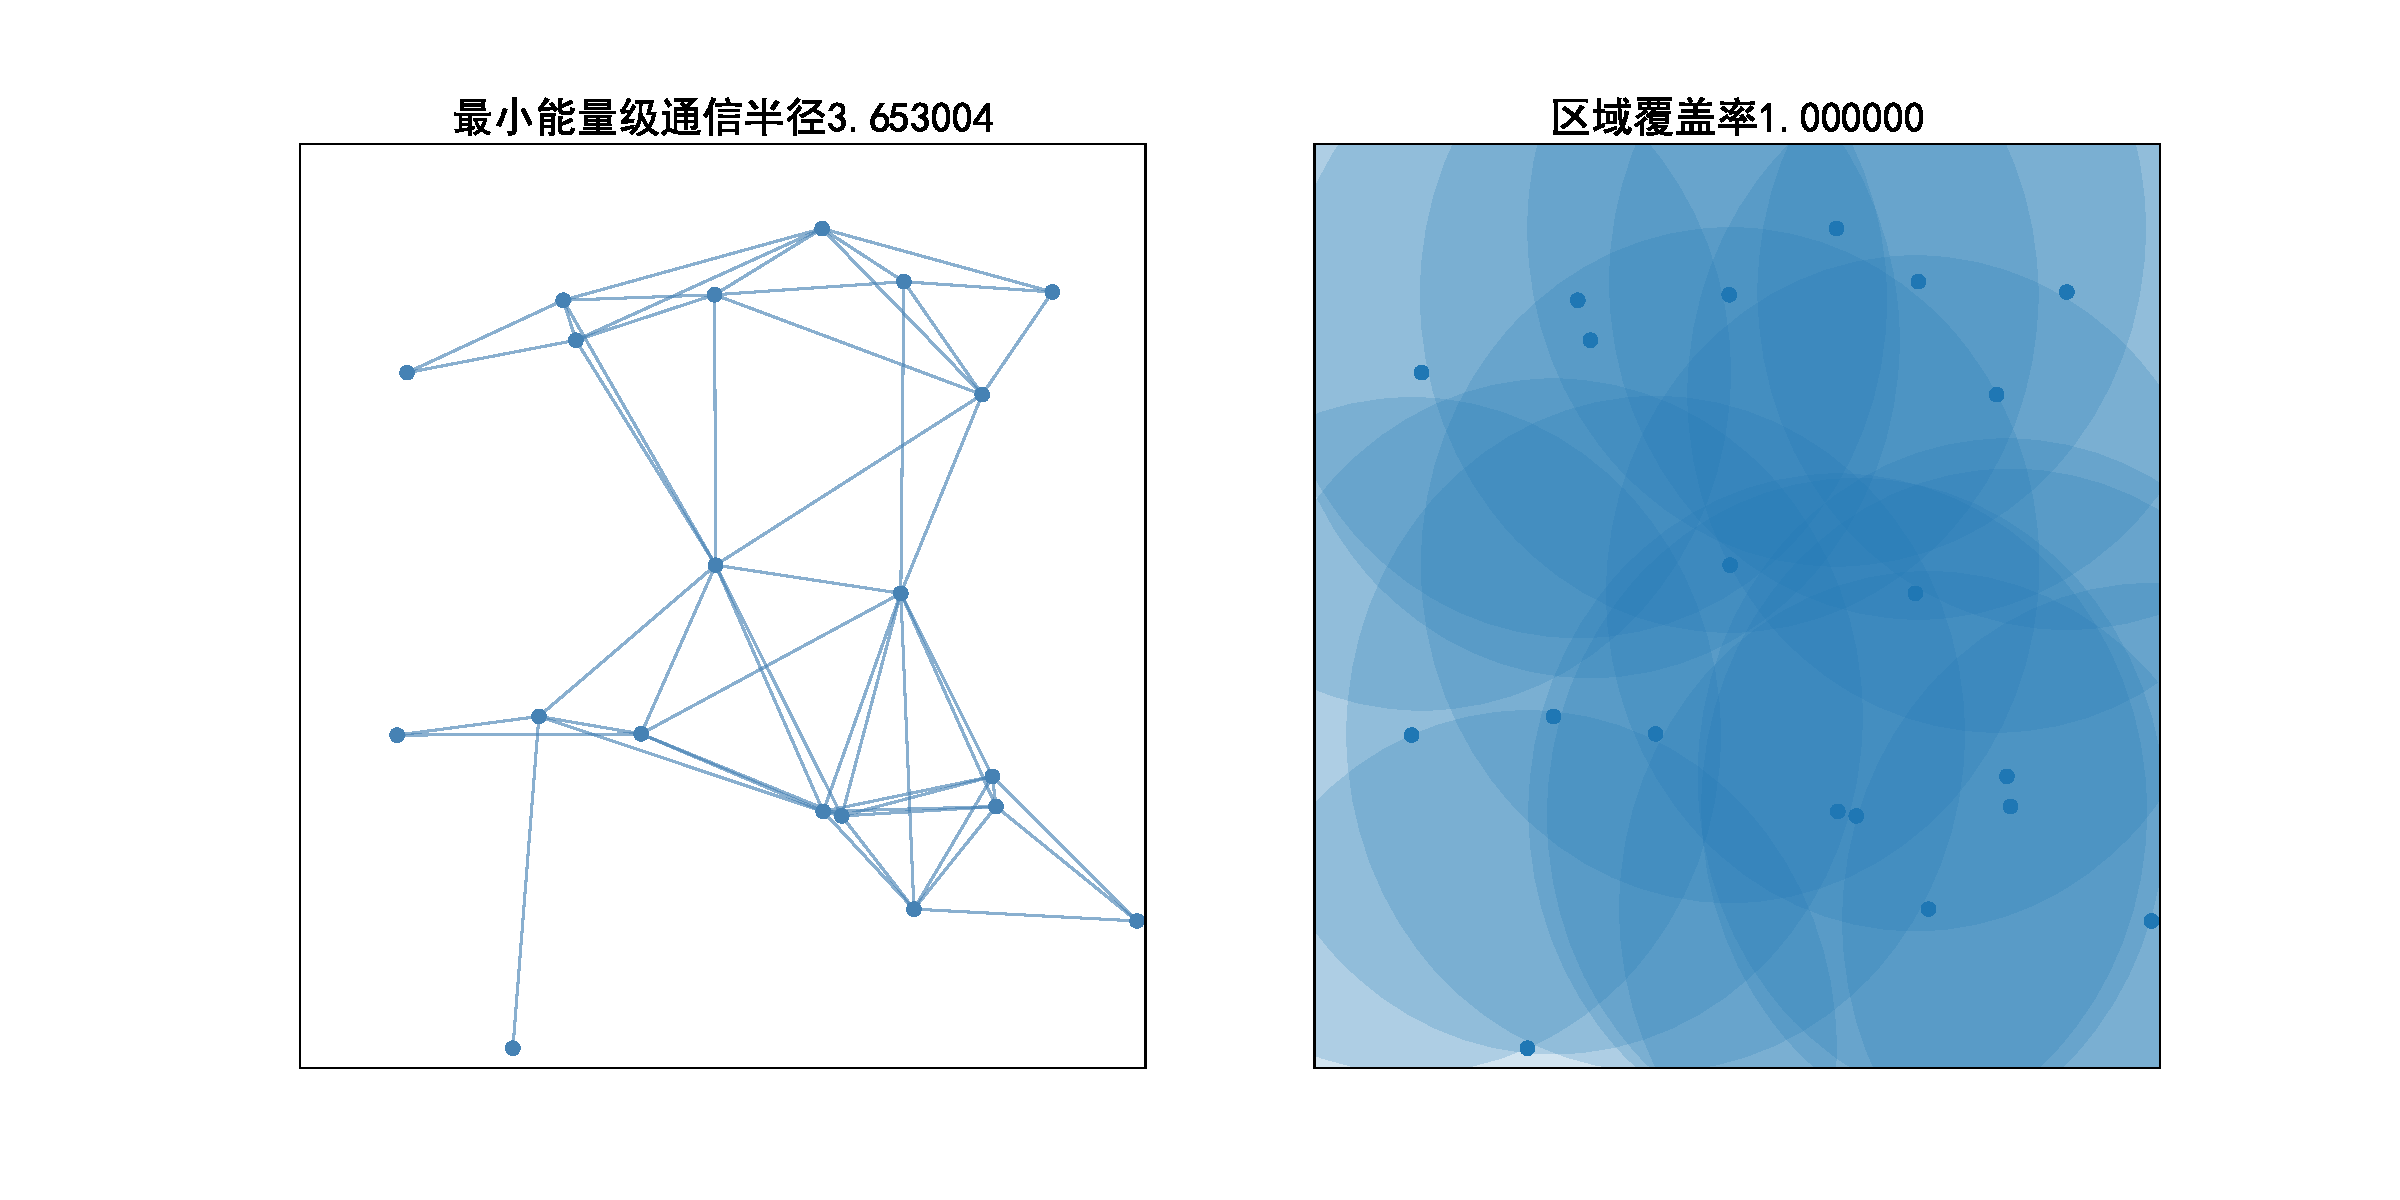
\includegraphics[width=\textwidth, keepaspectratio]{figure/f1/r_min.pdf}\\
				\caption{传感器数量$n=20$}\label{f1}
			\end{minipage}
			\hfill
			\hfill
			\begin{minipage}[htbp]{0.9\textwidth}
				\centering
				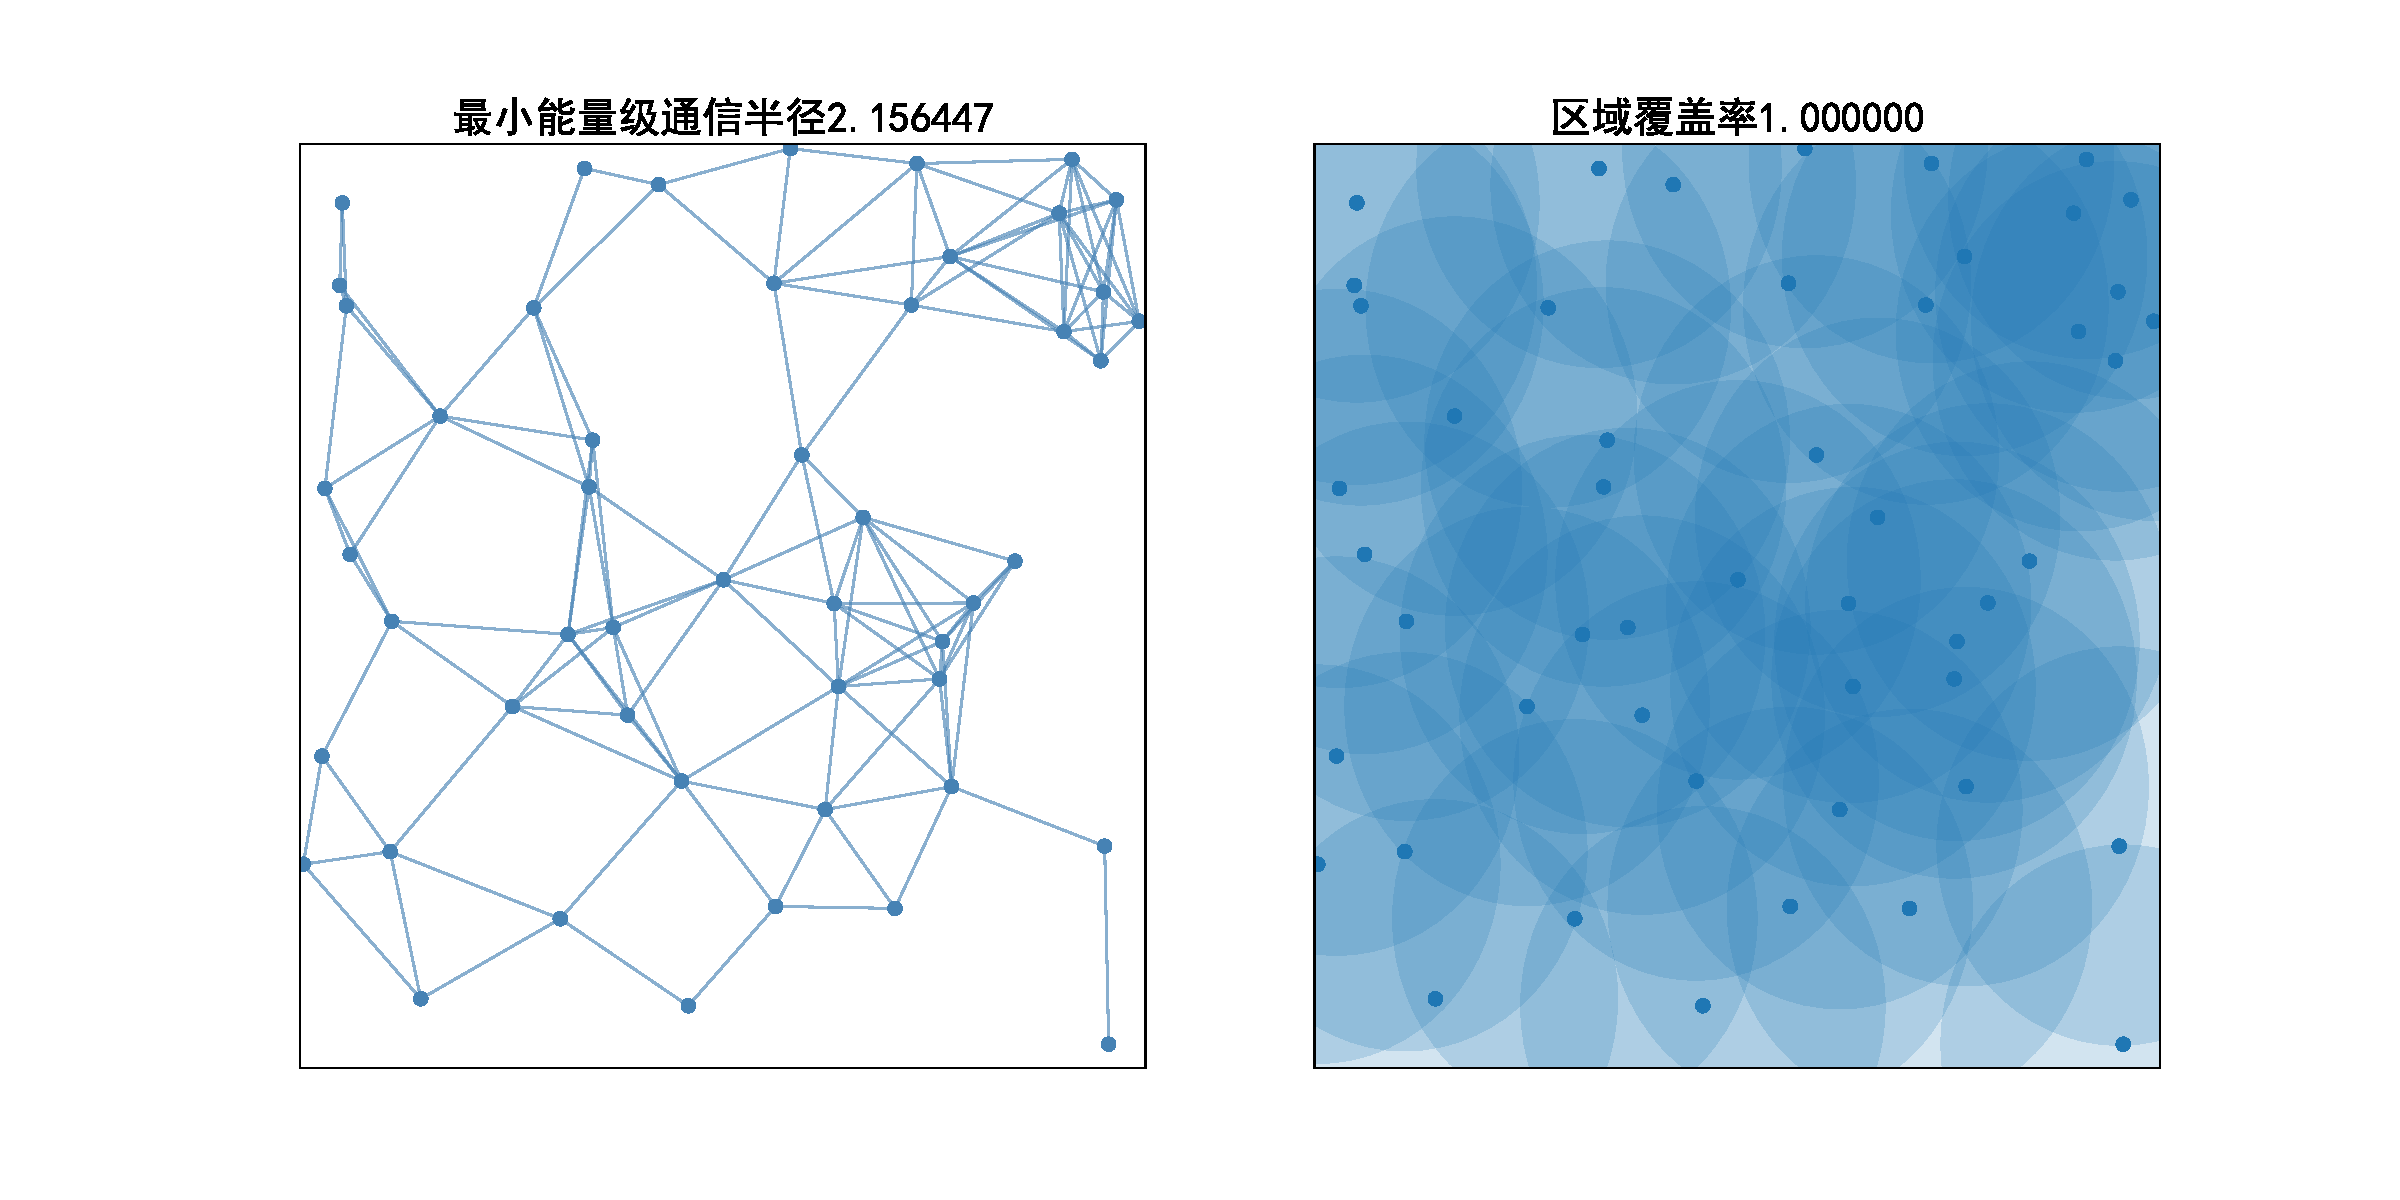
\includegraphics[width=\textwidth, keepaspectratio]{figure/f2/r_min.pdf}\\
				\caption{传感器数量$n=50$}\label{f2}
			\end{minipage}
		\end{figure}

	\section{实验结果分析}
	在COWPOW的运算过程中,对于任意给定的传感器节点分布,始终存在一个最小的通信半径$r_{min}$,使得当网络中节点的通信半径$r\ge r_{min}$时传感器网络中节点的连通性和网络以最大能量运行时的连通性相同。所以,为了节省能量,COWPOW协议以$r_{min}$为该网络的节点通信半径,从而确定网络对应的能量等级。
	
	对比图\ref{f1}和图\ref{f2}可知,区域大小一定,当传感器数量增多时,满足COWPOW协议的节点最小通信半径会上升;当传感器在区域内的分布较为均匀时,如果令节点覆盖半径等于满足COWPOW协议的节点最小通信半径,则区域内的传感器数量基本不会影响区域的覆盖率。
\end{spacing}
\end{document}